\subsection{Spettrometria $\gamma$}
Riassumiamo il principio di misura dell'energia del nostro spettrometro:
\begin{itemize}
	\item particelle cariche attraversano il cristallo scintillatore rilasciando energia all'interno per eccitazione/ionizzazione degli elettroni dello stesso;
	\item lo scintillatore produce luce in funzione dell'energia rilasciata ($\sim \SI{40}{fotoni \; keV^{-1}}$ nel NaI(Tl));
	\item i fotoni raggiungono il fotomoltiplicatore dopo essere stati riflessi sulle pareti del cristallo (rivestite di materiale riflettente) e nella guida ottica;
	\item il fotomoltiplicatore amplifica il segnale dei fotoni e produce in uscita un segnale (negativo e di breve durata: $\sim \SI{10}{\nano s}$) di picco proporzionale al numero di fotoni;
	\item la base del fotomoltiplicatore in dotazione fornisce anche un segnale pre-amplificato positivo a bassa impedenza (perciò di lunga durata $\sim \SI{1}{\micro s}$);
	\marginpar{Cosa vuol dire <<segnale a bassa impedenza>>?
	Se è il segnale di uscita è quello preamplificato
	quindi è banale dire che ha in qualche senso bassa impedenza di uscita
	e non implica che duri molto;
	se è il segnale in ingresso l'impedenza in ingresso del preamplificatore è invece alta
	e questo implica che il segnale duri più a lungo.\\
	\emph{Petrillo} \\
	Sulla scheda è scritto il contrario\\
	(Andrea)}
	\item questo segnale viene riconosciuto dal formatore/amplificatore che produce in uscita un segnale gaussiano di durata nota ($\SI{10}{\micro s}$) e di picco proporzionale all'energia rilasciata;
	\item l'output dell'amplificatore va all'ADC (tipicamente triggerato da un segnale esterno) che campiona sul massimo del segnale in una finestra temporale imposta dal trigger e converte il segnale in tensione in un segnale digitale a 13 bit.
\end{itemize}
Ciascuno di questi processi sarà caratterizzato da una:
\begin{itemize}
	\item\emph{funzione di risposta}: la funzione che da un certo input mi dà l'output medio (ad esempio energia della particella vs energia media rilasciata, energia rilasciata vs numero medio di fotoni prodotti, segnale in tensione vs digit, tutte in prima approssimazione lineari nel nostro range di lavoro\footnote{Discuteremo nel seguito la validità di questa approssimazione.});
    \item una \emph{distribuzione di risposta}: la distribuzione degli output a input fissato (ad esempio la distribuzione dei fotoni prodotti ad una energia fissata, queste ci aspettiamo avranno generalmente un forma a campana, in prima approssimazione gaussiana).
\end{itemize}
La misura finale avrà per funzione di risposta la composizione di tutte queste funzioni di risposta e per distribuzione di risposta la convoluzione delle distribuzioni di risposta (quest'ultima determinerà la risoluzione sperimentale).
\marginpar{Non è una convoluzione:
$p(x_0)=\int\de x_1 p(x_0|x_1) p(x_1)
=\int \de x_1 p(x_0|x_1) \int \de x_2 p(x_1|x_2)
=\int \de x_1 \dotsm \de x_n p(x_0|x_1)\dotsm p(x_{n-1}|x_n)$.\\
\emph{Petrillo}}

Nella nostra esperienza lo spettrometro dovrà misurare l'energia di fotoni $\gamma$ che, essendo neutri, devono prima interagire con la materia del rivelatore e trasferire tutta o parte della loro energia a particelle cariche, delle quali sarà poi misurabile l'energia nel modo descritto sopra. Bisogna quindi analizzare le interazioni fotone-materia per modellizzare gli spettri che andremo poi ad osservare.

%%%%%%%%%%%%%%%%%%%%%%%%%%%%%%%%%%%%%%%%%%%%%%%%%%%%%%%%%%%%%%%%%%%%%%%%%%%%%%%%%%%%

\subsubsection{Interazione fotone-materia}
I principali meccanismi di interazione dei fotoni con la materia sono:
\begin{itemize}
	\item assorbimento fotoelettrico;
	\item scattering Rayleigh;
	\item scattering Compton;
	\item produzione di coppie.
\end{itemize}
  
 \paragraph{Assorbimento fotoelettrico}
 Il fotone incidente è completamente assorbito e ionizza l'atomo, ovvero estrae un elettrone di energia cinetica 
 \begin{equation} \label{eq:fotoelettrico}
 T_e = E - E_b
 \end{equation} 
 dove $E$ è l'energia del fotone incidente e $E_b$ è l'energia di legame, solitamente piccola se paragonata a $E_{\gamma}$. Nel nostro caso l'energia di legame vale al massimo $\sim \SI{33}{keV}$ per gli elettroni 1s dello iodio, da confrontarsi con l'energia dei fotoni $\gamma$ del \co\;: \SI{1.17}{MeV} e \SI{1.33}{MeV}. Il risultato finale è una particella carica nello scintillatore con approssimativamente la stessa energia del fotone incidente.
 Un elettrone con energia cinetica di $\SI{1}{MeV}$ ha un range in NaI di $\sim \SI{2}{mm}$ (vedi \cite{3}), questo vuol dire che questi fotoni perdono tutta la loro energia nel nostro rivelatore (un cilindro retto $\sim \SI{5}{cm} \times \SI{5}{cm}$). 

 \paragraph{Scattering Rayleigh}
 Nello scattering Rayleigh l'intero atomo funge da bersaglio, perciò dopo l'urto il fotone cambia direzione e l'atomo rincula per conservare il momento. Data la grande massa dell'atomo (rispetto all'energia del fotone) l'energia scambiata è trascurabile e il fotone uscente ha praticamente la stessa energia iniziale. \`E chiaro quindi che i fotoni non potranno essere rivelati in uno scintillatore con questo meccanismo perché nessuna energia viene rilasciata all'interno.
 
 \paragraph{Scattering Compton}
 Se il fotone è abbastanza energetico può urtare un singolo elettrone. Per fotoni di questo tipo l'energia di legame può essere in prima approssimazione trascurata e si può trattare l'elettrone come libero. Nello stato finale troviamo il fotone che è stato deviato di un certo angolo $\theta$ rispetto alla sua direzione iniziale e ha ceduto parte della sua energia all'elettrone. La relazione tra energia del fotone dopo lo scattering e angolo è\footnote{Useremo la convenzione $e = c = 1$.}:
 \begin{equation}
 \label{energia_compton} 
 E'_{\gamma} = \frac{E_{\gamma}}{1+\frac{E_{\gamma}}{m_e}(1-\cos{\theta})}.
 \end{equation}
 Quello che misureremo nello spettroscopio sarà l'energia ceduta all'elettrone cioè $E-E'$. Quando un fotone fa scattering Compton nel nostro spettroscopio non abbiamo modo di conoscere l'angolo di scattering e non è possibile da una singola misura ricavare l'energia del fotone incidente.
 La sezione d'urto differenziale di questo processo (anche nota come formula di Klein–Nishina) è:
 \begin{equation}
 \label{klein-nishina}
 \frac{d\sigma}{d\cos{\theta}} = \frac{\pi\text{Z}}{m_e^2} \cdot\left(\frac{E'_{\gamma}}{E_{\gamma}}\right)^2 \cdot \left(\frac{E_{\gamma}}{E'_{\gamma}} + \frac{E'_{\gamma}}{E_{\gamma}} - \sin^2{\theta}\right),
 \end{equation}
 dove $\frac{E'}{E}$ contiene implicitamente l'angolo attraverso la \eqref{energia_compton}.
 La sezione d'urto differenziale è graficata in \autoref{fig:klein-nishina}
 \marginpar{In che unità di misura è la sezione d'urto in figura?
 Metterlo nella caption.\\
 \emph{Petrillo}}
 ed è da qui evidente come all'energia di $\sim \SI{1}{MeV}$ è molto più probabile che il fotone sia deviato poco, tuttavia esiste un angolo critico per cui l'energia ceduta dal fotone non è sufficiente a ionizzare e di fatti l'elettrone non può più considerarsi libero. L'energia di legame dell'orbitale K del carbonio (il materiale del nostro bersaglio) vale $E_b = \SI{0.277}{keV}$ e per i fotoni del \co\; l'angolo critico vale $\theta_c \simeq \SI{0.8}{\degree}$. 
 
 \begin{figure}[h]
 	\centering
 	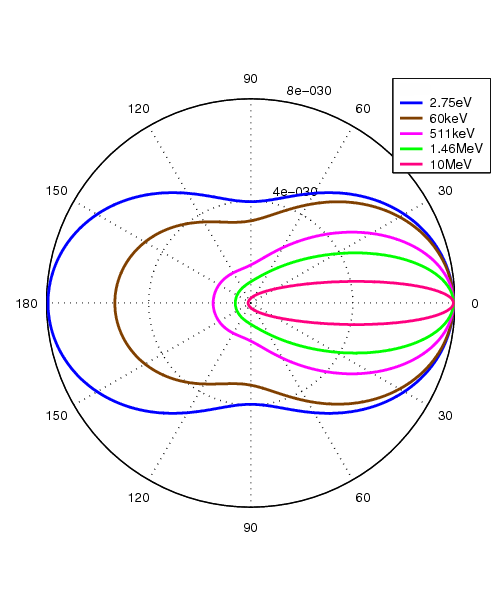
\includegraphics[width=20em]{klein-nishina}
 	\caption{\label{fig:klein-nishina}Sezione d'urto in funzione dell'angolo di scattering Compton.}
 \end{figure}

 \paragraph{Produzione di coppie}
 Il fotone $\gamma$ può fare scattering con un fotone del campo e.m. del nucleo (o meno probabilmente di un elettrone) e produrre una coppia $e^+e^-$. Affinché questo processo sia accessibile cinematicamente l'energia del fotone deve essere maggiore di \SI{1.02}{MeV}, quindi questo processo è possibile per i fotoni del \co\;  e del \na, tuttavia, come vedremo, questo processo è largamente trascurabile a queste energie, rispetto agli altri in gioco.
 
 %%%%%%%%%%%%%%%%%%%%%%%%%%%%%%%%%%%%%%%%%%%%%%%%%%%%%%%%%%%%%%%%%%%%%%
 
 \subsubsection{Sezione d'urto fotone-materia} \label{efficiency}
 La sezione d'urto fotone-materia per ciascuno dei processi prima descritti dipenderà dallo Z del materiale. In generale a basse energie ($ < \SI{10}{keV}$) sarà dominante l'assorbimento fotoelettrico, ad alte energie ($>\SI{100}{MeV}$) predominerà la produzione di coppie mentre lo scattering Compton sarà dominante in un range intermedio. L'estensione di questo range è maggiore al diminuire di Z come è chiaro dalla \autoref{fig:photon_cross_section_pdg}.
 
  \begin{figure}[h]
 	\centering
 	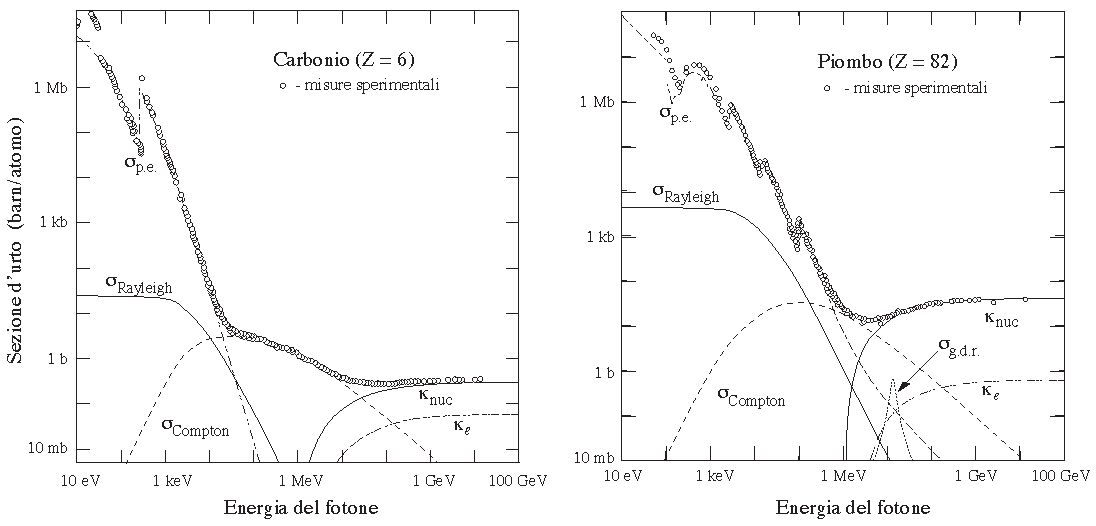
\includegraphics[width=\textwidth]{photon-matter-interaction}
 	\caption{\label{fig:photon_cross_section_pdg}Sezione d'urto in funzione dell'energia per i vari processi nel carbonio e nel piombo \cite{4}}
 \end{figure}

 \paragraph{Scelta del materiale per bersaglio e spettrometro}
 Nella nostra esperienza il bersaglio sarà di carbonio, mentre lo spettrometro è un cristallo di NaI ($\text{Z}(\text{Na})=11$, $\text{Z}(\text{I})=53$). Questa scelta è giustificata dal fatto che nel carbonio, all'energia dei fotoni del \co{}, la sezione d'urto dell'assorbimento fotoelettrico è ampiamente trascurabile e l'energia del fotone è più facilmente misurabile dai fotopicchi associati all'assorbimento fotoelettrico. Sarà perciò preferibile usare il cristallo di NaI come spettrometro poiché a $\sim\SI{1}{MeV}$ il rapporto tra sezione d'urto Compton e sezione d'urto dell'assorbimento fotoelettrico vale circa 20, come si può vedere in \autoref{fig:photon_cross_section_xcom}. Questo è sufficiente per rendere i fotopicchi chiaramente visibili con la risoluzione strumentale. Inoltre scegliendo il carbonio per il bersaglio  sarà garantito che tutti i fotoni che interagiranno nel carbonio lo faranno per effetto Compton.
  
  \begin{figure}[h]
 	\centering
 	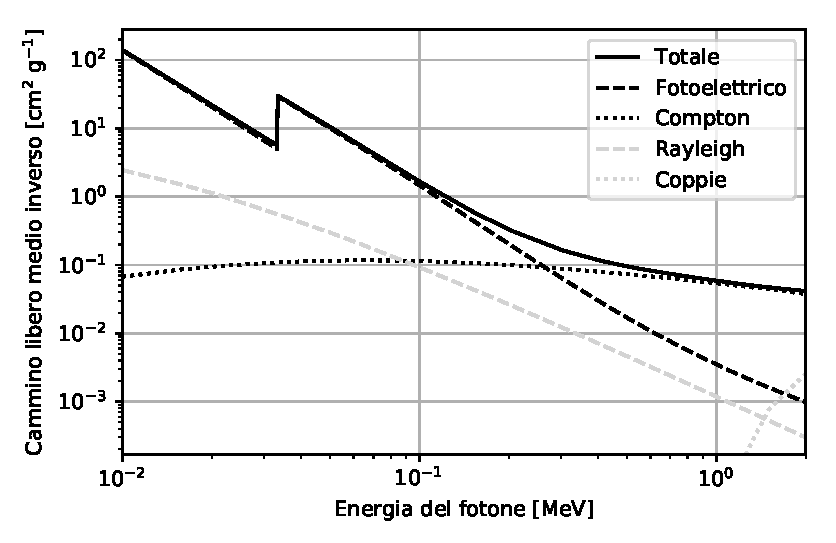
\includegraphics[width=30em]{cross}
 	\caption{\label{fig:photon_cross_section_xcom}
	Sezione d'urto del fotone in funzione dell'energia per i vari processi nel NaI,
	espressa come inverso del cammino libero medio diviso per la densità del materiale
	e moltiplicato per la sezione d'urto relativa \cite{5}. La densità del NaI è \SI{3.67}{g\,cm^3}.}
 \end{figure}
 \marginpar{non è il cammino libero medio inverso}
 %%%%%%%%%%%%%%%%%%%%%%%%%%%%%%%%%%%%%%%%%%%%%%%%%%%%%%%%%%%%%%%%%%%%%%%%
 \subsubsection{Spettri attesi e dimensione del detector}
 \paragraph{Grande detector} Se il detector fosse abbastanza esteso, tutta l'energia dei fotoni, indipendentemente dalla complessità dell'interazione, verrebbe rilasciata nel rivelatore. Per una sorgente di fotoni ad una energia fissata, come potrebbe essere una sorgente di raggi $\gamma$\footnote{I raggi $\gamma$ delle sorgenti radioattive hanno tipicamente larghezze $\Gamma \ll \SI{1}{eV}$ e possono quindi considerarsi mono-energetici per i nostri scopi.},
 \marginpar{Non si dice monocromatici piuttosto che mono-energetici?\\
 \emph{Petrillo}}
 ad esempio il \cs, lo spettro energetico prodotto da un tale scintillatore sarebbe un singolo fotopicco all'energia dei fotoni $\gamma$ (vedi \autoref{fig:spettrometro_grosso}) con una larghezza dovuta essenzialmente alla risoluzione dello strumento, come analizzeremo nel seguito.
 
 \begin{figure}[h]
 	\centering
 	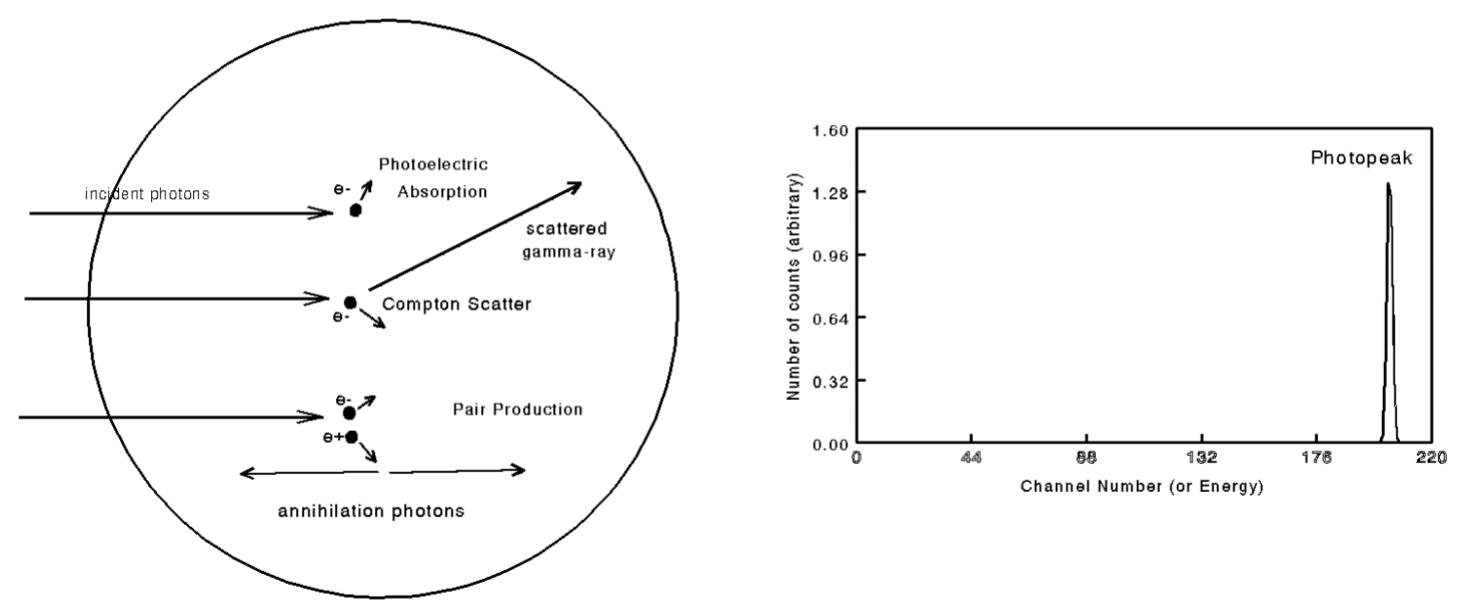
\includegraphics[width=\textwidth]{spettrometro_grosso}
 	\caption{\label{fig:spettrometro_grosso}
	Risposta di un detector di grandi dimensioni per fotoni mono-energetici \cite{6}.}
 \end{figure}

 \paragraph{Piccolo detector}Nel caso opposto di un detector di piccole dimensioni i fotoni potranno interagire una sola volta, facendo effetto fotoelettrico o Compton\footnote{Stiamo trascurando la produzione di coppie, per i motivi detti sopra.} in proporzione alla sezione d'urto. I fotoni che fanno effetto fotoelettrico produrranno un segnale alla loro energia (che non sarà una delta ma sarà allargato dalla risoluzione strumentale) come visto prima, mentre i fotoni che faranno fotoelettrico si produrranno uno spettro come quello predetto dalla sezione d'urto di Klein-Nishina (la spalla Compton sarà meno definita perché convoluta con la risoluzione strumentale).
\marginpar{Non credo che sia una convoluzione perché la $\sigma$ della gaussiana dipende dall'energia.\\
\emph{Petrillo}}
Il risultato finale sarà simile a quelli in \autoref{fig:spettrometro_piccolo}.
 
  \begin{figure}[h]
 	\centering
 	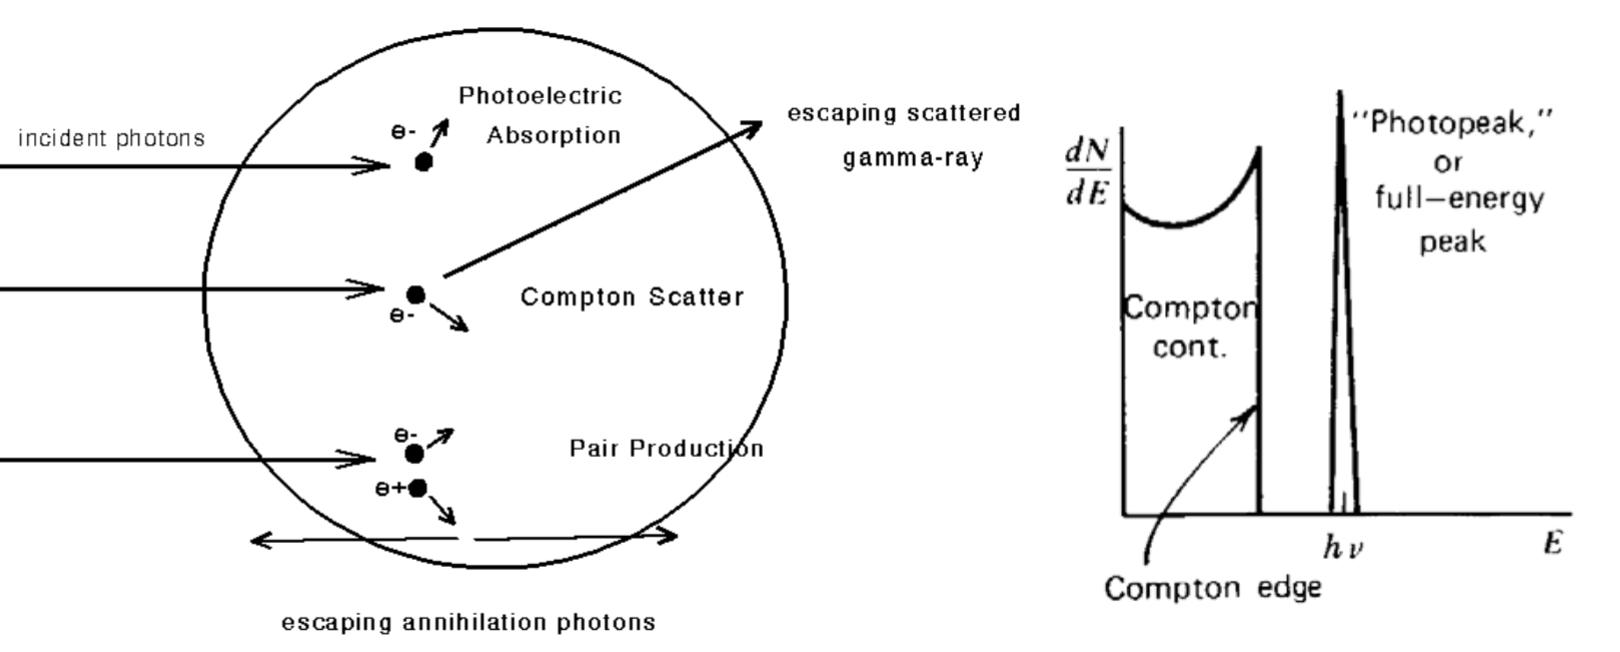
\includegraphics[width=\textwidth]{spettrometro_piccolo}
 	\caption{\label{fig:spettrometro_piccolo}Risposta di un detector di piccole dimensioni per fotoni mono-energetici \cite{6}.}
 \end{figure}
 
 \paragraph{Detector di dimensioni intermedie}\label{par:spettrometro_intermedio}
 Nel nostro caso disponiamo di un rivelatore $\SI2{''}\times\SI2{''}$ e, a partire dal grafico in \autoref{fig:photon_cross_section_xcom}, è semplice calcolare che per il nostro rivelatore la lunghezza di radiazione è circa \SI{5}{cm}, quindi paragonabile alla dimensione del cristallo, ne segue che il $\sim \SI{60}\%$ dei fotoni interagisce nel cristallo almeno una volta. Ci troviamo quindi in una situazione intermedia per cui in pratica lo spettro sarà simile a quello in \autoref{fig:spettrometro_piccolo}, ma il rapporto tra gli eventi Compton e quelli fotoelettrico non sarà uguale al rapporto tra le sezioni d'urto: è infatti importante il contributo di quei fotoni che dopo aver fatto Compton fanno fotoelettrico\footnote{Questa doppia interazione è anche favorita dal fatto che i fotoni che hanno fatto scattering Compton hanno perso energia e l'effetto fotoelettrico ha sezione d'urto maggiore al diminuire dell'energia.} (quando ancora si trovano nello spettrometro): questi produrranno un segnale all'energia del fotopicco poiché tutta l'energia del fotone iniziale è rilasciata nello scintillatore. 
 
 Lo spettro finale prodotto sarà la somma di molti effetti riassunti in \autoref{fig:spettrometro_intermedio}:
 \begin{itemize}
 	\item l'assorbimento fotoelettrico produrrà un fotopicco all'energia dei fotoni incidenti;
 	\item i fotoni che fanno scattering Compton rilasceranno solo parte della loro energia producendo il caratteristico profilo predetto dalla  formula di Klein-Nishina;
 	\item i fotoni che fanno scattering Compton sui materiali che circondano il detector possono tornare nello stesso producendo un picco, detto di backscattering nella regione a basse energie;
 	\item spesso potrebbe essere visibile un picco all'energia caratteristica dei raggi X emessi dai materiali circostanti (ad esempio lo stesso spettrometro);
 	\item se la sorgente decade $\beta^+$ (come il \na) sarà visibile un fotopicco a \SI{511}keV dovuto ai fotoni $\gamma$ prodotti nell'annichilazione del positrone con la materia circostante.
 \end{itemize}
Lo spettro finale atteso (per una sorgente che emetta un solo fotone e uno spettrometro di dimensioni intermedie) è schematizzato in \autoref{fig:spettrometro_intermedio} e si può confrontare con un tipico spettro acquisito con il nostro spettrometro in \autoref{fig:spettro_tipico} (si tratta del \cs\; che emette un fotone a \SI{662}keV).

 \begin{figure}[h]
	\centering
	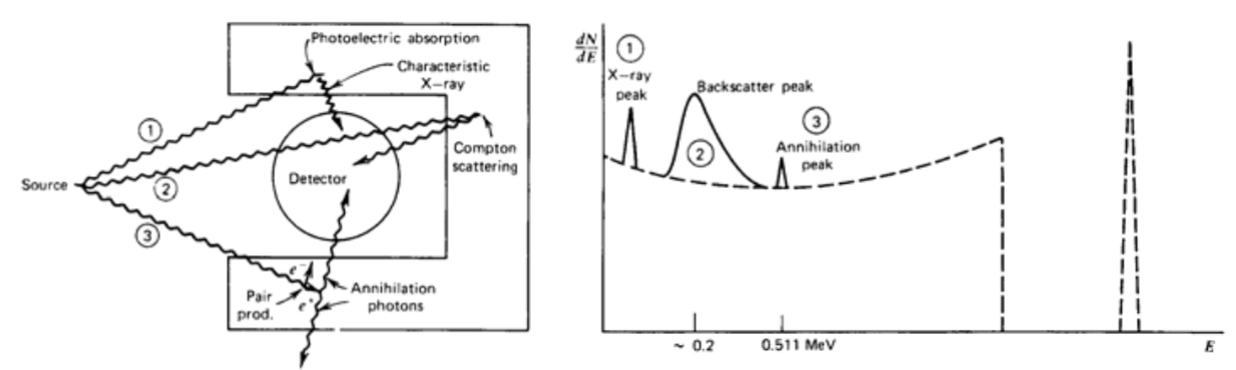
\includegraphics[width=\textwidth]{spettrometro_intermedio}
	\caption{\label{fig:spettrometro_intermedio}Risposta di un detector di dimensioni intermedie (come il nostro) per fotoni mono-energetici \cite{6}.}
 \end{figure}

 \begin{figure}[h]
	\centering
	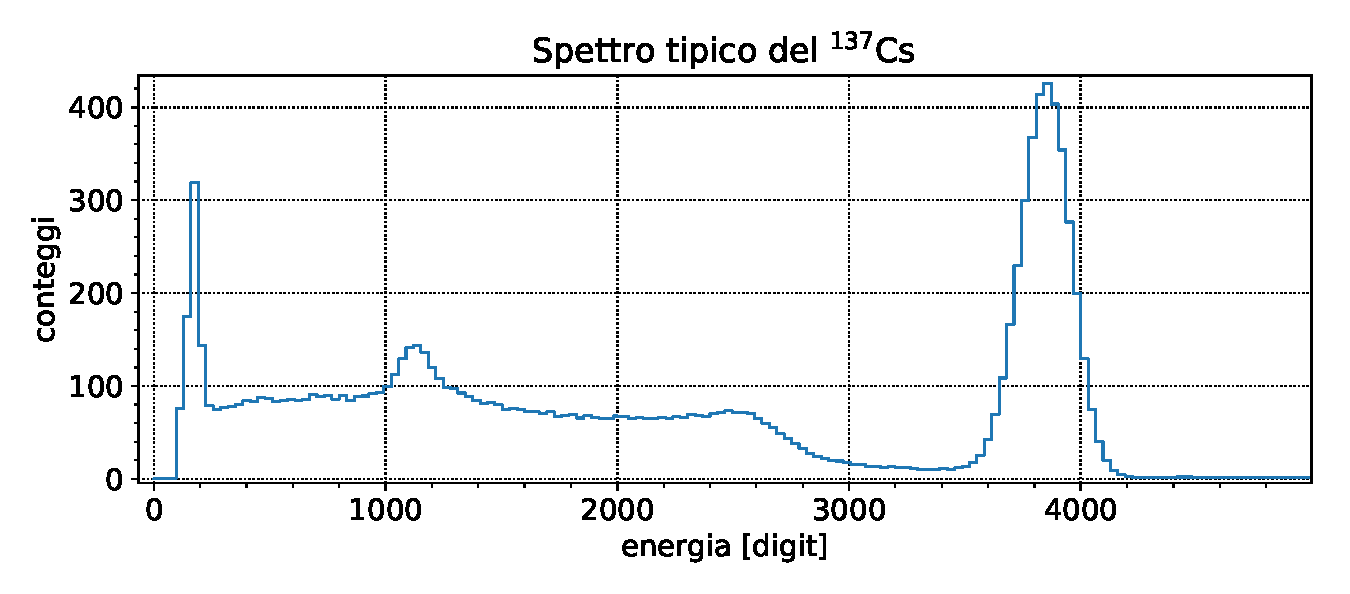
\includegraphics[width=\textwidth]{spettro_tipico}
	\caption{\label{fig:spettro_tipico}Un tipico spettro (\cs) acquisito con il nostro rivelatore. Si possono notare da sinistra verso destra: il picco dei raggi X, quello del backscattering, la spalla Compton e il fotopicco principale.}
\end{figure}

\marginpar{La qualità di \autoref{fig:spettrometro_intermedio} è talmente bassa che non riesco a leggerla nemmeno se la ingrandisco \\ (Andrea)}

 %%%%%%%%%%%%%%%%%%%%%%%%%%%%%%%%%%%%%%%%%%%%%%%%%%%%%%%%%%%%%%%%%%%%%%%%%%%%%%%%
 \subsubsection{Risposta del detector e calibrazione}
 Poiché ci troviamo nel caso descritto in \autoref{par:spettrometro_intermedio} non è possibile misurare l'energia di un singolo fotone $\gamma$ con il nostro apparato; l'unico modo per effettuare una misura di energia è supporre una certa distribuzione di energia della sorgente\footnote{I fotoni prodotti dalle nostre sorgenti radioattive sono monocromatici ai nostri scopi, lo stesso non si può dire dei fotoni secondari prodotti dallo scattering Compton sul nostro bersaglio e del quale vogliamo misurare l'energia, per questi dovremo ricavare la distribuzione in energia.} e fittare con uno spettro atteso.
 Il modo più semplice è fittare il fotopicco che per sua natura sarà centrato all'energia dei fotoni incidenti (a meno di una correzione dovuta all'energia di legame che non è trascurabile a basse energie), alternativamente si può fittare la spalla Compton, che tuttavia è molto più difficile da modellizzare e dipende dalla massa dell'elettrone, la cui misura è l'obiettivo di questa esperienza. Nel seguito quindi quando ci riferiremo a funzioni e distribuzioni di risposta ci riferiremo alla sola posizione e forma del fotopicco.

 \paragraph{Efficienza}
 In definitiva un fotone che attraversa il cristallo di NaI può: 
 \begin{itemize}
 	\item non interagire con probabilità $e^{-\frac{L}{\lambda}}$ dove $L$ è la distanza percorsa nel cristallo (che sarà dell'ordine dei \SI{5}{cm}) e $\lambda$ è la lunghezza di attenuazione (che nel nostro caso è dell'ordine dei \SI{5}{cm});
 	\item fare effetto Compton con probabilità $(1-e^{-\frac{L}{\lambda}})\cdot \frac{\sigma_{C}(E)}{\sigma_\text{tot}(E)}$ dove $\sigma_{C}(E)$ è la sezione d'urto Compton all'energia $E$ e $\sigma_\text{tot}(E)$ è la sezione d'urto totale alla stessa energia;
 	\item fare effetto fotoelettrico con probabilità $(1-e^{-\frac{L}{\lambda}})\cdot \frac{\sigma_\text{ph}(E)}{\sigma_\text{tot}(E)}$.
 \end{itemize}
 Il fotone uscente dal Compton ha quindi le stesse possibilità di interazione ma con probabilità calcolate alla nuova energia e sulla nuova distanza percorsa.\marginpar{questo è un po' una ripetizione di roba già detta, ma mi sembrava il caso di ricapitolare (Bob)}
 Il fatto che le sezioni d'urto cambino al variare dell'energia\footnote{Sopratutto quella dell'effetto fotoelettrico che nella regione di energie di interesse è molto ripida come si vede in \autoref{fig:photon_cross_section_xcom}.} e quindi l'efficienza di rivelazione produrrà una deformazione della spettro osservato.
 
\marginpar{Proporrei (e quindi l'efficienza di rivelazione) in modo che non si possa fraintendere \\ (Andrea)}
 
 Nella misura dell'energia dei fotoni secondari, l'efficienza di rivelazione nel NaI è anche correlata all'angolo di scattering poiché i fotoni che deviano di un angolo piccolo cedono poca energia agli elettroni del bersaglio, perciò l'efficienza di rivelazione nel bersaglio diminuisce e conseguentemente quella della coincidenza.
 
 \paragraph{Funzione di risposta (linearità)}
 Un rivelatore di radiazione ideale dovrebbe essere lineare. Come già detto la funzione di risposta del nostro spettrometro è la composizione delle funzioni di risposta dei singoli processi prima elencati e ci aspettiamo che alcune di queste devino da un comportamento puramente lineare, ad esempio
 \begin{itemize}
 	\item la funzione di risposta associata all'interazione dei fotoni per effetto fotoelettrico è affine come visto in \autoref{eq:fotoelettrico}, dove per $E_b$ prendiamo l'energia di legame media;
 	\item è noto che la luce di scintillazione per i detector in NaI non è proporzionale all'energia depositata, come mostrato in figura \autoref{fig:linearità}.
 \end{itemize}
 Poiché l'energie che andremo a misurare saranno tutte nel range \SI{500}keV--\SI{1300}{keV}, range nel quale la risposta dello scintillatore è ragionevolmente lineare, decidiamo di fittare la risposta dello spettrometro con una retta a intercetta libera, usando tutti i fotopicchi a disposizione tranne quello del \am{} che emette fotoni a \SI{60}keV, lontani dalla regione di interesse e di linearità.
 
 \begin{figure}[h]
	\centering
	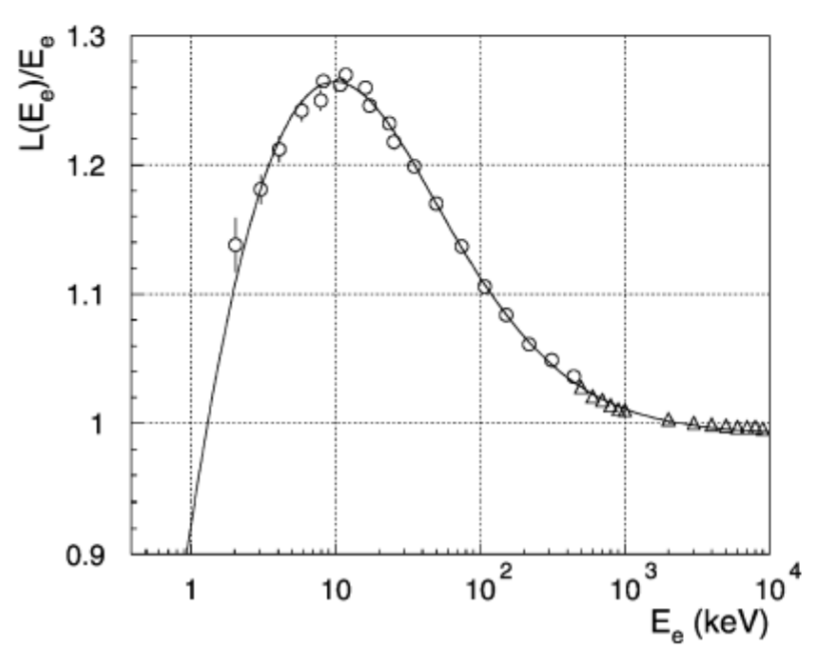
\includegraphics[width=20em]{linearita}
	\caption{\label{fig:linearità}Numero relativo di fotoni emessi dal cristallo di NaI(Tl) vs energia degli elettroni \cite{6}.}
 \end{figure}
 
 \paragraph{Distribuzione di risposta (risoluzione)}
 La distribuzione di risposta sarà quindi la forma del fotopicco. Per sorgenti monocromatiche e trascurando momentaneamente il fondo della spalla Compton\footnote{Il modello scelto per i fondi verrà trattato in \autoref{par:fondo1} e \autoref{par:fondo2}.} decidiamo di considerare un modello gaussiano con varianza che dipenderà dall'energia.
 I fotoni secondari che dal bersaglio arrivano allo spettrometro non sono monocromatici ma hanno una certa distribuzione dovuta all'accettanza angolare dello spettrometro e alla divergenza angolare del fascio di fotoni. Sarà necessario quindi simulare la distribuzione dei fotoni secondari considerando il fondo della spalla Compton e l'allargamento dovuto a accettanza angolare, divergenza del fascio e risoluzione strumentale.
 
 